\clearpage
\subsection{Program (with functions)} % (fold)
\label{sub:program_with_functions_}

You can declare your own Functions within the program's code.

\begin{figure}[h]
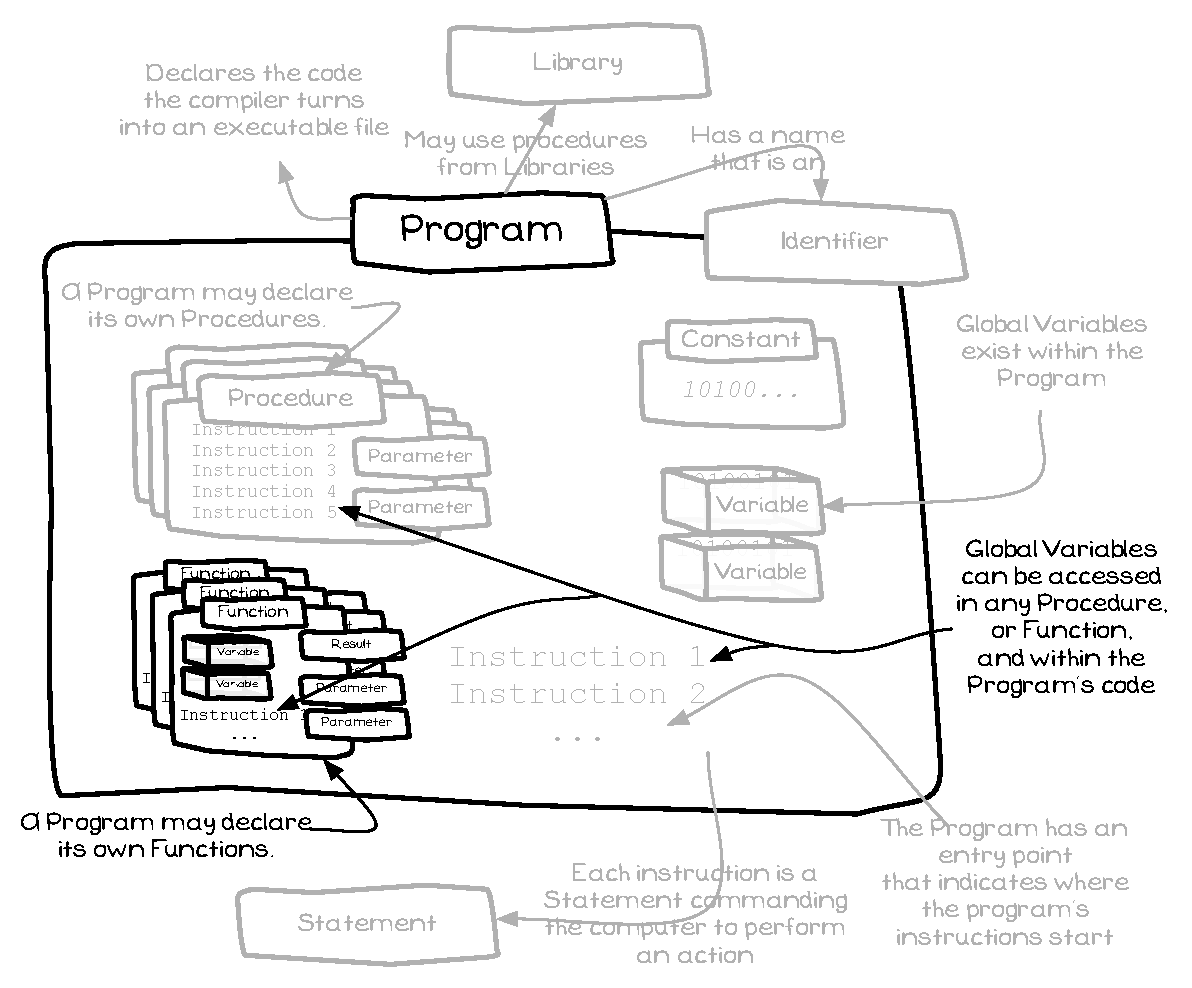
\includegraphics[width=\textwidth]{topics/storing-using-data/diagrams/ProgramWithFunctions} 
 \caption{You can declare your own Functions in your program's code}
 \label{fig:function-decl-programs}
\end{figure}

\mynote{
\begin{itemize}
  \item A Program is an \textbf{Artefact}, you create Programs that the user can execute. Internally these programs contain other artefacts such as Procedures, Functions, and Variables.
  \item You can declare your own \nameref{sub:function}s within your program's code.
  \item With C and Pascal the Function must be declared before it is used.
\end{itemize}
}

% subsection program_with_functions_ (end)